\section{Marketing}
\label{section_marketing}
Das Marketing hat neben dem typischen Aufgabenbereich der Außenrepräsentation durch die Besonderheiten einer Hochschule auch einen Aufgabenbereich der Innenrepräsentation. Im folgenden werden diese Bereiche getrennt betrachtet.

\subsection{Externes Hochschulmarketing}
\label{subsection_externes_hochschulemarketing}
Das externe Marketing der Hochschule bezieht sich auf die klassischen Marketingaufgaben, das Produkt und die Marke vorteilhaft darzustellen. Im Falle einer Hochschule ist dies die attraktive Darstellung gegenüber zukünftige Studierenden, Forschungsinteressierten und Geldgebern.

\subsubsection{Webseite}
Zentrales Element bleibt die Hochschulwebseite, die mit aktuellen, offenen Möglichkeiten von HTML 5, CSS 3 und JavaScript den Funktionsumfang einer App erreichen kann, ohne auf spezielle oder spezifische Spezialtechnologien zu setzen. Besonders sei an dieser Stelle die Möglichkeit genannt, mittels CSS Größen und Darstellungsmöglichkeiten von Endgeräten unabhängig von konkreten Betriebssystemen und Hardwareplattformen abzudecken.

Dies ist vor dem Hintergrund wichtig, dass beispielsweise eine native App für iPhones zwingend durch den Appstore der Firma Apple installiert werden muss, dessen Nutzungsbedingungen sich für die Hochschule in Form von Kosten oder Inhaltseinschränkungen zu Ungunsten der Hochschule verändern könnten. Mit einer nativen App lässt sich trotzdem nur ein beschränkter Nutzerkreis ansprechen. Sollen mehrere Apps für verschiedene Plattformen gepflegt werden, so ist dies mit zusätzlichen Aufwand verbunden.

Eine Neuauflage der Hochschulwebseite mit aktuellen Möglichkeiten und per CSS an verschiedene Darstellungsgrößen angepasst erreicht dagegen jedes internetfähige Gerät mit Browser. Sollte ein neuer Formfaktor wichtig werden, zum Beispiel der einer Smartwatch, so lässt sich dies über eine Erweiterung des Stylesheets erreichen, ohne eine komplette Neuentwicklung in Auftrag zu geben.

\subsubsection{Soziale Netzwerke}
Soziale Netzwerke wie facebook oder twitter sind kritisch zu bewerten. Auftritte auf diesen Plattformen können nicht alleine stehen, benötigen aber durch ständigen Nutzerkontakt eigenständige Pflege und Aufsicht, was an einer kleinen Hochschule Personal bindet.

Der Nutzen ist weiterhin fraglich. Die Hochschule kann bestenfalls Informationen der Webseite duplizieren, während Kommunikation von Interessierten zur Hochschule wieder schnell in bestehende Kanäle geleitet wird.

Weiterhin ist die Reichweite zwar potentiell weltweit, was für eine nach Leitbild „Hochschule der Region“ aber an sich nicht relevant ist. In der Praxis wichtiger ist die Dichte der Nutzer, da es unrealistisch ist zu erwarten, dass jeder in sozialen Netzwerken organisiert ist, oder aber sich zur Nutzung in einem sozialen Netzwerk anmelden müsste.

Über interne Kommunikation und Daten in sozialen Netzwerken müsste im Einzelfall nach Grundlage geltender Datenschutzvorgaben entschieden werden, was als Prozess vorab bereits zu aufwendig, als dass eine Erwägung hier weiter Sinn machen würde.
Im Endeffekt verbliebe also die Verbreitung ohnehin öffentlicher Informationen, die bereits auf der Webseite zu finden wären.

\subsubsection{Verteilte Content-Erzeugung}
Im Kontext einer kleinen Hochschule ist die Personalsituation zu berücksichtigen. Es kann nicht davon ausgegangen werden, dass eine oder mehrere Personen die Redaktion aller zu veröffentlichenden Inhalte übernehmen. Vielmehr ist zu erwarten, dass relevante Neuigkeiten an mehreren unterschiedlichen Stellen auftreten, und am besten ohne Umweg veröffentlicht werden. Hierzu eignen sich Content-Management-Systeme.

\begin{figure}[h!]
	\centering
	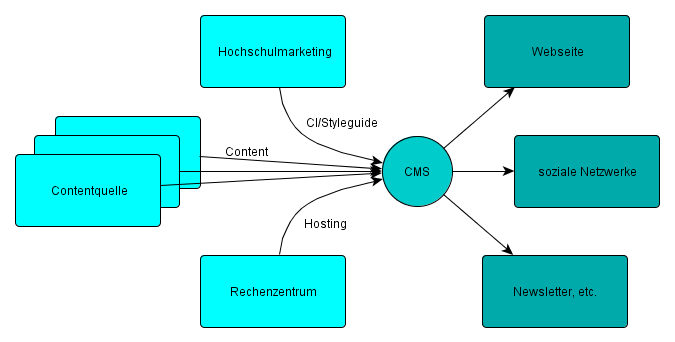
\includegraphics[width=10cm]{kapitel/gruppe3/bilder/verteilter_publishing_workflow}
	\caption{Verteilter Publishing Workflow}
	\label{fig_publishing_workflow}
\end{figure}

Mit diesen kann geleistet werden, dass mehrere, unabhängige Autoren Inhalte beisteuern und veröffentlichen können, ohne im Einzelnen mit den technischen Einzelheiten des Hostings oder des Designs belangt zu werden. Auch können vielfach Content Management Systeme Inhalte für weitere Plattformen aufbereiten, zum Beispiel an soziale Netzwerke posten.

\subsection{Internes Hochschulmarketing}
\label{subsection_internes_hochschulemarketing}
Im Gegensatz zur Situation in einem Unternehmen genießen einzelne Fachbereiche und Personen in einer Hochschule einen hohen Grad an Freiheit und Autonomie. Daher können in Arbeitsgruppen und Gremien beschlossene Prozesse und Software nicht per Anordnung durchgesetzt werden, sondern müssen nach innen vermarktet werden, um akzeptiert zu werden.Herausfordernd ist hier besonders die Heterogenität, da der technische und fachliche Hintergrund sich unter Mitarbeitern und Fachbereichen erheblich unterscheiden dürften, etwa zwischen technischen und nichttechnischen Fachbereichen.

\subsubsection{Fokussierter Support}
Eine Möglichkeit, Benutzer hin zu einer präferierten Lösung zu leiten ist diese in Präferenzen, Anleitungen und FAQs an erster Stelle und in höherem Detailgrad zu präsentieren. Vielfach wird eine Voreinstellung einfach übernommen, und die erste Lösung zu einer Fragestellung als Referenz angesehen.

\subsubsection{Schulungen}
Eine weitere Maßnahme ist, Schulungen für die präferierten Lösungen anzubieten, die Vorteile der gefundenen Lösung gegenüber anderen herausstellt. Optimal ist eine solche Lösung transparent, oder aber bietet Alleinstellungsmerkmale, die eine Verwendung aus sich heraus attraktiv erscheinen lassen. Trotzdem kann es vorkommen, dass in Lern- und Umstellungsphasen Lernkurven in der Benutzung absolviert werden müssen. Soll eine Lösung akzeptiert werden, dann muss diese Lernkurve entsprechend begleitet werden.

\subsubsection{Integration}
Eine weitere starke, aber arbeitsintensive Maßnahme ist, die präferierte Lösung stark zu integrieren. Beispielsweise sei die Erstellung von hochwertigen Dokumentvorlagen entsprechend der Corporate Identity für die präferierte Textverarbeitung genannt.

Der Übergang zum fokussierten Support ist hier fließend. Wird die präferierte Lösung an das bestehende System angepasst, so kann von Integration gesprochen werden, wird das System an eine präferierte Lösung angepasst, ist dies fokussierter Support. Beides kann sehr gut gegenseitig ergänzend eingesetzt werden.